% =================================================================================================
\chapter{Aplikacija}
% =================================================================================================
Jedan od glavnih ciljeva ovog rada je kreiranje aplikacije, koja bi vršila poređenje izlaza iz prediktora i metodom konsenzusa dala procenu, koja bi pomogla u utvrđivanju neuređenih regiona sekvence.  \\

U nastavku je detaljno opisana izrađena aplikacija sa svim važnim aspektima koji je čine. Programski jezici korišćeni za izradu ovog projekta su \textbf{JavaScript} i \textbf{Python}, a za izradu samôg interfejsa korišćene su veb tehnologije \textbf{HTML} i \textbf{CSS}.
% -------------------------------------------------------------------------------------------------
\section{Arhitektura}
% -------------------------------------------------------------------------------------------------
Arhitekturalna organizacija aplikacije je $klijent-server$ arhitektura. Klijent-server arhitektura podrazumeva odvajanje uloga: klijenta, koji zahteva neku uslugu od servera, i servera, koji tu uslugu pruža i šalje odgovor klijentu. Ovaj vid arhitekture je odabran kako bi se jasno razdvojile uloge između klijenta koji komunicira sa korisnikom i servera koji komunicira sa prediktorima.

\subsection{Klijent} 
Klijent je implementiran u vidu korisničkog interfejsa, koji od korisnika aplikacije zahteva određene unose. Ti unosi se, potom, šalju serveru na obradu.\\\\
Od unosa na klijentskoj strani zahtevaju se \textit{identifikator} u \textit{DisProt} bazi i sekvenca, koja je opciona. Na osnovu identifikatora, sekvenca se, ukoliko nije uneta, povlači iz baze, a ukoliko identifikator nije unet, program izbacuje obaveštenje da ga je obavezno uneti. Sekvenca se unosi u \textit{.fasta} formatu, klikom na dugme $"$browse$"$ ili kao sirova niska kroz tekstualno polje. Klikom na dugme $"$submit$"$ uneti podaci se šalju na server gde se obrađuju. Klijent ostatak vremena izvršavanja programa osluškuje i čeka na odgovor od servera. Prikaz izgleda korisničkog interfejsa može se videti na slici \ref{fig:interfejs}.\\\\
\begin{figure}[H]
	\centering
    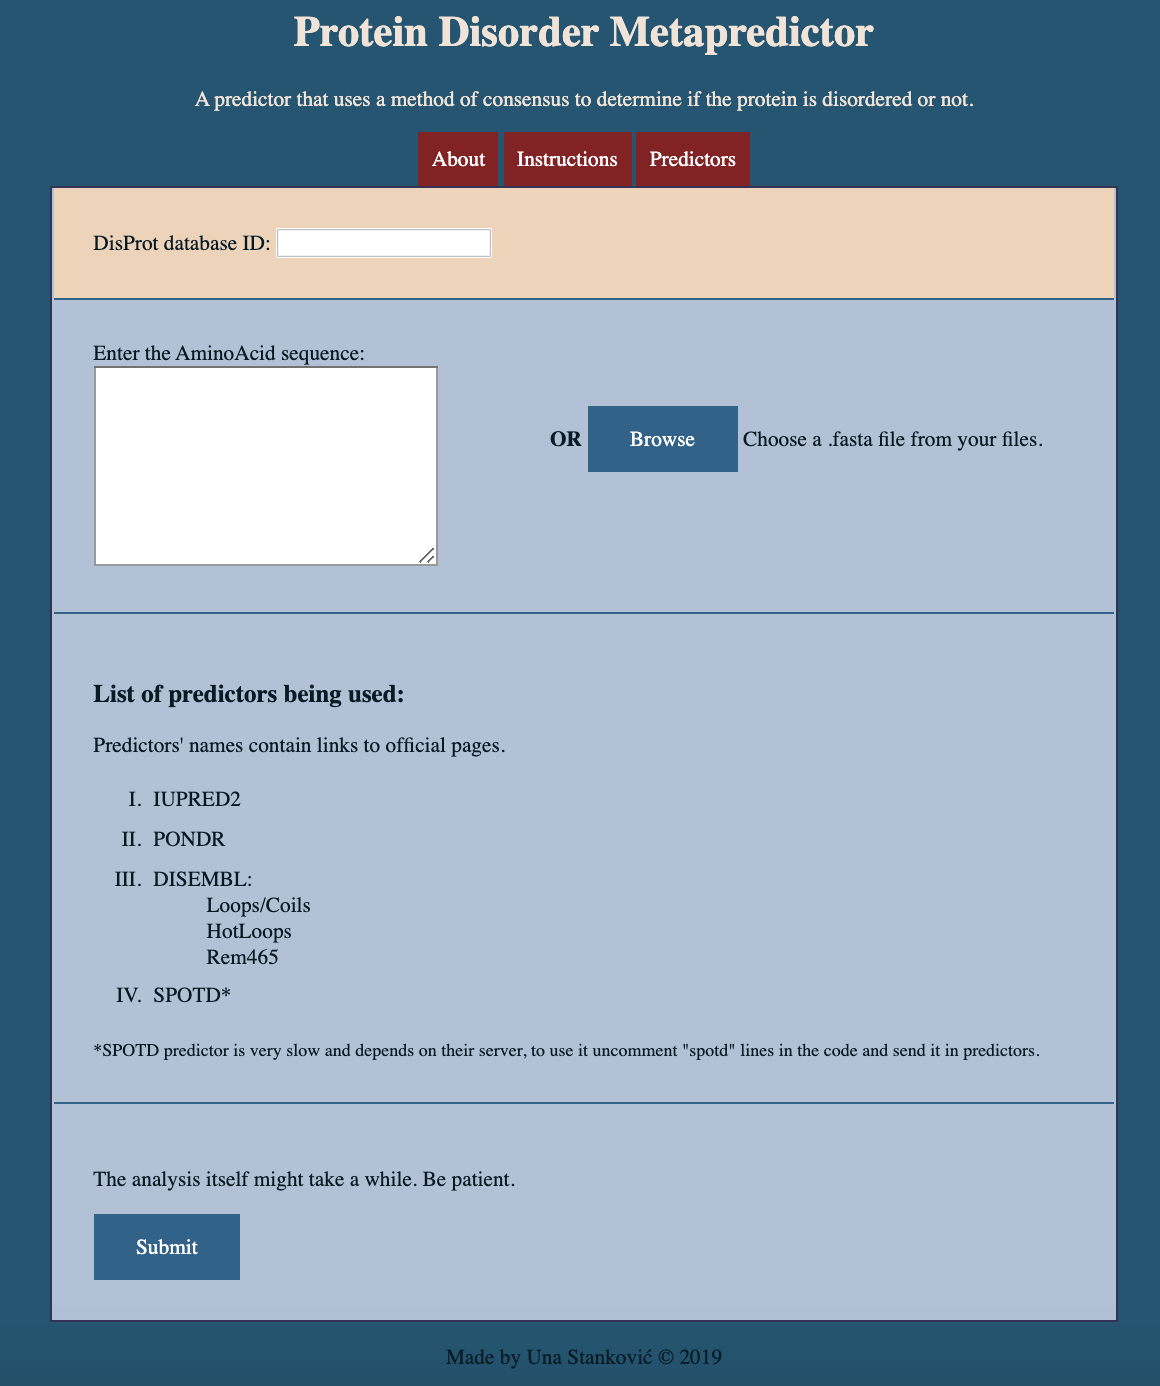
\includegraphics[width=0.7\textwidth]{Figures/App/interfejs.png}
    \caption{Prikaz korisničkog interfejsa.}
    \label{fig:interfejs}
\end{figure}

Nakon što server obradi podatke, rezultati se vraćaju klijentu i prikazuju se u vidu nekoliko nizova. Ti nizovi predstavljaju izlaze prediktora, odnosno, njihove odluke o uređenosti (neuređenosti) svake od aminokiselina u sekvenci. U prvom redu predstavljena je sekvenca, aminokiselina po aminokiselina. U ostalim redovima predstavljeni su slovom $"$D$"$ neuređeni regioni sekvence. Na osnovu \textit{identifikatora} u \textit{DisProt} bazi određuju se eksperimentalno neuređeni regioni, koji se nalaze u pretposlednjem redu,  obeleženi, takođe, slovom $"$D$"$ . U poslednjem redu se nalazi konsenzus prediktora (proračunat na osnovu odgovora prediktora, podrazumevano bez korišćenja informacija iz $DisProt$ baze.). Potom, prikazane su vrednosti metrika ispod kojih se nalazi grafički prikaz konsenzusa nad niskom sa pragom od $0.5$ i skalom datih rezultata na $y$-osi.  \\ 
Na samom kraju, nalazi se tabela koja sadrži podatke o metrikama u zavisnosti od broja prediktora koji su rekli da je region neuređen. Posmatra se sledeće tvrđenje: $"$ \textit{Aminokiselina je neuređena ukoliko je $k$ prediktora reklo da je neuređena}.$"$ \\ 
Prikaz stranice sa rezultatima može se videti na slici \ref{fig:rezultati}.
\begin{figure}[H]
	\centering
    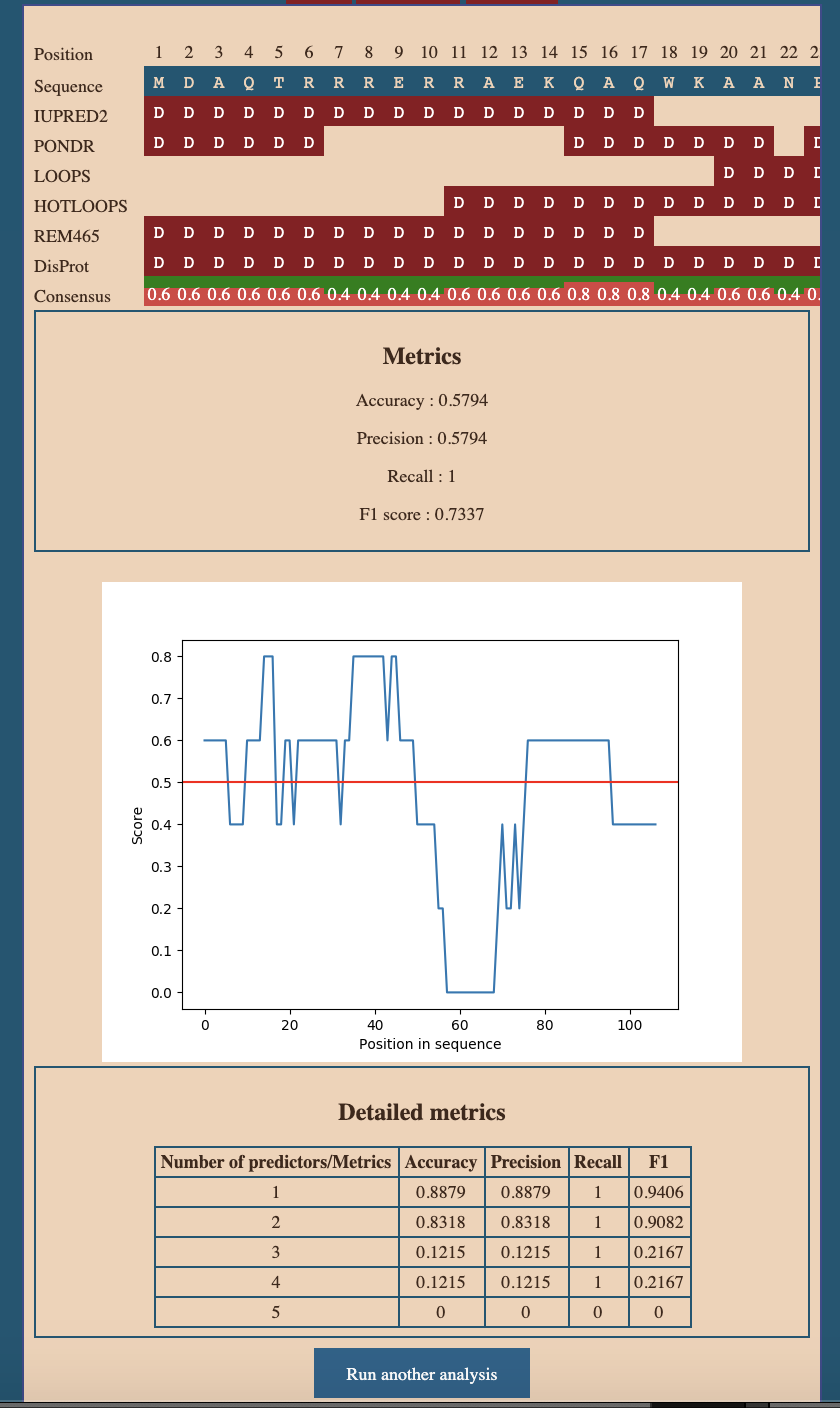
\includegraphics[width=0.7\textwidth]{Figures/App/rezultati.png}
    \caption{Prikaz korisničkog interfejsa pri povratku rezultata sa servera za protein sa identifikatorom $DP00005$.}
    \label{fig:rezultati}
\end{figure}

\subsubsection{Implementacija klijenta}
Klijent je implementiran kroz skriptni programski jezik $"$JavaScirpt$"$ i korišćenjem veb tehnologija $HTML5$ i $CSS3$. 
Ceo kôd klijenta sastoji se iz narednih datoteka:
\begin{itemize}
\item \textbf{index.html} - glavna strana koja od korisnika zahteva unos i sadrži informacije o projektu, uputstvo za korišćenje aplikacije, kao i informacije o prediktorima,
\item \textbf{style.css} - datoteka sadrži sve stilove korišćene kroz aplikaciju,
\item \textbf{sock\_cli.js} - datoteka prikuplja informacije unete od strane klijenta i prosleđuje ih serveru i prima informacije od servera i poziva funkcije iz $results.js$ kako bi se izvršio prikaz dobijenih rezultata na stranici,
\item \textbf{results.js} - datoteka sadrži funkcije za kreiranje prikaza i vrši prikaz dobijenih rezultata na stranici dinamički, kreiranjem novih elemenata, 
\item \textbf{loader.js} - datoteka menja prikaz stranice prilikom čekanja na server.
\end{itemize}

Za komunikaciju sa serverom koristi se $socketio$ biblioteka. Podaci se šalju emitovanjem određenog događaja čiji se naziv navodi kao prvi argument funkcije $emit$.
\begin{lstlisting}[language=Python]
const socket = io('http://localhost:5000');
socket.on('connect', () => {
    console.log('Connected to server');
});

function sendData() {
    if (txtDisprotId.value == ""){
        alert("You must enter the DisProt id!");
    }
    else{
        showLoader();
        const json = generateData();
        console.log('Sending to server.');
        socket.emit('message', json);
    }
}
\end{lstlisting}

Primanje podataka vrši se reagovanjem na događaj koji se navodi kao prvi argument funkcije $on$. Kako bi se podaci pravilno prikazali  više funkcija za prikaz različitih delova rezultata moraju biti pozvane.

\begin{lstlisting}[language=Python]
socket.on('predicted', data => {
    console.log('Got from server.');
    console.log(data);
    createScale(data.sequence);
    for (const pred of data.predictors) {
        createPredictor(pred.result, pred.name);
    }
    hideLoader(); 
    createConsensus(data.consensus.result);
    addMetrics(data.metrics);
    addDetailedMetrics(data.partial_metrics);
});
\end{lstlisting} 

\subsection{Server} 
 Serverska obrada se sastoji iz komunikacije sa lokalno čuvanim aplikacijama (programima za prediktore), kao i postojećim veb stranicama kako bi se obezbedili podaci neophodni za analizu.\\
 
Serveska strana komunicira sa klijentskom stranom korišćenjem soketa, odnosno $socketio$ biblioteke. Ovaj vid komunikacije u kombinaciji sa nitima, je odabran zbog čekanja na izlaze iz predikotra. Ukoliko bi se radilo o nekom drugom vidu komunikacije moglo bi da se desi da se rezultati ne prikažu ili izmešaju zbog neujednačenog vremena povratka informacija. Server slušanjem čeka na informacije od klijenta i po primanju informacija vrši nekoliko radnji:
\begin{itemize}
\item  \textit{DisProt}  \textit{identifikator} šalje se zahtevom preko omogućenog $API$-ja\footnote{API - skraćeno od engl. \em{Application Programming Interface}, predstavlja interfejs za komunikaciju sa, u ovom konkretnom slučaju, $DisProt$ $bazom$. }. Odgovor se potom parsira regularnim izrazima kako bi se dobili eksperimentalno neuređeni regioni - intervali regiona u sekvenci i sekvenca. Potom se ti intervali popunjavaju u listi i ona se vraća kao niz karaktera $"$D$"$ i $"$-$"$, gde $"$D$"$ predstavlja neuređenost.
\item Sekvenca se smešta u zasebnu datoteku, za potrebe lokalno čuvanih prediktora. Osim toga, sekvenca se dodatno parsira (ukoliko je u $.fasta$ formatu onda se iz nje uklanja prva linija, kako bi bila prilagodjena za ulaz prediktorima koji zahtevaju samo sirovu sekvencu).
\item Sekvenca se šalje prediktorima. Prediktori su kreirani kao elementi klase $Predictor$ i za svaki od njih se računa $calculate$ funkcija koja vraća listu karaktera $"$D$"$ i $"$-$"$.
\item Svaki od prediktora prima sekvencu i na poseban način je obrađuje:
	\begin{itemize}
	\item \textit{IUPRED2} - Prediktor se nalazi lokalno sačuvan i prosleđuje mu se naredba za pokretanje, kao i naziv datoteke u kojoj je sačuvana niska koja se obrađuje.  
	\item \textit{PONDR} - Prediktor se nalazi na $web$  \href{http://www.pondr.com/cgi-bin/pondr.cgi}{lokaciji} na kojoj se nalazi forma koja se dinamički popunjava na osnovu korisničkog unosa uz pomoć $mechanize$ modula. Potom se regularnim izrazom parsira dobijeni rezultat.  
	\item \textit{SPOTD} - Prediktor se nalazi na $web$ \href{http://sparks-lab.org/server/SPOT-disorder/}{lokaciji} i postupak je poput prethodnog prediktora, međutim, problem koji se javlja sa ovim prediktorom je taj što je server poprilično spor (izvršavanje preko 10 minuta, server često nije dostupan). Za korišćenje ovog prediktora neophodno je skinuti komentare iz koda i dodati u $predictors$ objekat rezultat $spotd$ predikcije.
	\item \textit{DISEMBL} - Prediktor predstavlja spoj tri prediktora $coils/hotcoils$, $loops$ i $rem465$ . Prediktor se nalazi na $web$ \href{http://dis.embl.de/cgiDict.py}{lokaciji}. Ovaj prediktor vraća rezultate na osnovu tri vida predikcije. 
	\end{itemize}
\end{itemize}

\subsubsection{Implementacija servera}
Serverska strana je u potpunosti implementirana u programskom jeziku $Python$ i organizovana je kroz sledeće datoteke:
\begin{itemize}
\item \textbf{sock\_serv.py} - Datoteka sadrži srž serverske strane programa. U datoteci su organizovani primanje informacija sa servera i emitovanje povratnih informacija. 
\item \textbf{predictor\_service.py} - Datoteka sadrži kreiranje elemenata klasa i vraća izračunate vrednosti predikcije.  
\item \textbf{disprot\_service.py} -U ovoj datoteci se nalazi povezivanje na   \textit{DisProt} bazu i parsiranje dobijenih rezultata. Iz dobijenih informacija iz baze zanimaju nas intervali koji sadrže neuređene regione i sekvenca. Iako su pored regiona obezbeđene informacije o metodu kojim su oni određeni, za ovaj rad ti podaci nisu relevantni. 
\item \textbf{predictor.py} - Datoteka sadrži kreiranu klasu prediktor, i metode koje su neophodne za svaki od prediktora.  
\item \textbf{consensus.py} - Datoteka sadrži funkcije vezane za kreiranje konsenzusa i iscrtavanje rezultata.
\item \textbf{measures.py} - Datoteka sadrži funkcije vezane za formiranje metrika. 
\item \textbf{pondr.py}  
\item  \textbf{spotd.py}  
\item \textbf{iupred2.py}  
\item \textbf{disembl.py}  
\end{itemize}
Poslednje navedene datoteke sadrže informacije opisane u prethodnoj podeli, svaki rezultat je predstavljen u vidu liste. 

Za komunikaciju sa klijentom, koristi se $socketio$ biblioteka, koja funkcioniše po istom principu kao na klijentskoj strani. Konekcija sa klijentom:

\begin{lstlisting}[language=Python]
sio = socketio.Server(cors_allowed_origins=['http://localhost:9004'])
app = socketio.WSGIApp(sio, static_files={
    '/': {'content_type': 'text/html', 'filename': 'index.html'}
})

@sio.event
def connect(sid, environ):
    print('connect ', sid)
    
if __name__ == '__main__':
    eventlet.wsgi.server(eventlet.listen(('', 5000)), app)
\end{lstlisting}

Primanje informacija od klijenta funkcioniše tako što server sluša čekajući na poruku i po prijemu poruke poziva funkciju za pozivanje prediktora.
\begin{lstlisting}[language=Python]
@sio.on("message")
def message(sid, data):
    print('message ', data)
    
    # Calling all the predictors to give their opinion on the sequence in the same thread!
    x = threading.Thread(target=prediction_calls(data), args=(data))
    x.start()
\end{lstlisting}

Funkcija za pozivanje prediktora se sastoji iz nekoliko celina:
\begin{enumerate}
\item Najpre se iz prosleđenih podataka izvlače informacije o $identifikatoru$ i $sekvenci$ ako postoji. 
\begin{lstlisting}[language=Python]
def prediction_calls(data):
    id_disp = data["disprot_id"]
    s = data["sequence"]
    # DisProt database call
    [disprot, seq] = disprot_service.get_sequence_info(id_disp)
    print(seq, len(seq))
    if (s == ""):
        s = seq
\end{lstlisting}
Oni se prosleđuju $get\_sequence\_info$ u datoteci $disprot\_service.py$ koja dohvata informacije iz baze. Pripremanje sekvence sastoji se iz parsiranja povratnih informacija sa servera, izvlačenja intervala i popunjavanja pozicija tih intervala sa $"$D$"$.
\begin{lstlisting}[language=Python]
def get_sequence_info(id_disp):
   # response = requests.get('http://www.disprot.org/ws/get/' + id_disp) # Old API changed on 13.09.2019.
    response = requests.get('http://www.disprot.org/api/' + id_disp)
    data = json.loads(response.content)
    if re.search("200", str(response)) == None:
        data = "Not found."
    return prepare_sequence(data)
    
def prepare_sequence(data):
    if data == "Not found.":
        return data
    sequence = data['sequence']
    seq_len = len(shortened_sequence(sequence)) 
    intervals = []
    disprot = []
    disprot = ['-'] * seq_len
    for record in data['regions']:
        start_interval = record["start"]
        end_interval = record["end"]
        intervals.append((start_interval, end_interval))
    for interval in intervals:
        begin, end = int(interval[0]), int(interval[1])
        for i in range(begin-1, end):
            disprot[i] = "D"
    return disprot, sequence
\end{lstlisting}

\item Potom se sekvenca čuva lokalno u fajlu.
\begin{lstlisting}[language=Python]
 # Storing the sequence in a file in order to locally use the predictors
    f = open("sequence.txt", "w")
    f.write(s)
    f.close()
\end{lstlisting}
\item Nakon toga pozivaju se prediktori da pojedinačno daju rezultat. Prediktor $SPOTD$ je izuzet iz računanja, jer zavisi od njihovog servera koji je često nedostupan ili veoma spor (izračunavanje traje više od 15 minuta). 
\begin{lstlisting}[language=Python]
# Calling predictors
    iupred2 = predictor_service.iupred2_predict(s)
    #SPOTD: uncomment the function call 
    #spotd = predictor_service.spotd_predict(s) 
    pondr = predictor_service.pondr_predict(s)
    ss = shortened_sequence(s)
    [loops, hotloops, rem465] = predictor_service.disembl_predict(ss)
\end{lstlisting}
Prilikom poziva prediktora, unutar funkcija oblika $nazivprediktora\_predict$, kreira se instanca klase $Predictor$ za datu sekvencu, a vraća se izračunat rezultat predikcije. Navedene funkcije nalaze se u datoteci $predictor\_service.py$.
\begin{lstlisting}[language=Python]
def iupred2_predict(sequence):
    p = iupred2(sequence)
    return p.calculate()

def spotd_predict(sequence):
    p = spotd(sequence)
    return p.calculate()

def pondr_predict(sequence):
    p = pondr(sequence)
    return p.calculate()

def disembl_predict(sequence):
    p = disembl(sequence)
    return p.calculate() 
\end{lstlisting}
Izgled klase $Predictor$ iz datoteke $predictor.py$.
\begin{lstlisting}[language=Python]
class Predictor:
    def __init__(self, sequence):
        self.sequence = sequence
        self.calculated = []

    def calculate(self):
        pass # Store result in self.calculated in form [aa1_prediction, aa2_prediction, aa3_prediction, ...]
\end{lstlisting}
Za prediktore kojima se pristupa preko njihovih veb stranica koristi se biblioteka $mechanize$ za popunjavanje odgovarajućih formi i biblioteka $re$ kojom se uvode regularni izrazi, neophodni za parsiranje dobijenih rezultata. Primer jednog od prediktora kod koga se predikcija vrši preko veb stranice:
\begin{lstlisting}[language=Python]
class pondr(Predictor):
    def calculate(self):
      global br
      url = "http://www.pondr.com/cgi-bin/pondr.cgi" 
      br.set_handle_robots(False)
      br.open(url)
      br.form = list(br.forms())[1] 
      br['ProteinName'] = "test"
      br['Sequence'] = self.sequence 
      response = br.submit()
      soup = BeautifulSoup(response.read(), features='html5lib')
      soup = soup.prettify()
      result = re.findall("VLXT\t\s.*", soup)
      # We don't need the first one because it is not sequence
      result = result[1:]
      predicted = []
      for r in result:
          pred = r[6:]
          predicted.append(pred)
      total = []
      # Getting everything in one sequence 
      for i in predicted:
        total += i
      old = len(total)
      
      pom = shortened_sequence(self.sequence)
      if(old < len(self.sequence)):
        for i in range(0,len(pom) - old):
          total.append(" ")
      total = [x if x != ' ' else '-' for x in total ]
      
      self.calculated = total
      return self.calculated
\end{lstlisting}
\item Računa se konsenzus, a potom se računaju metrike uz pomoć funkcije $measure\_all$ koja se nalazi u datoteci $measure.py$. 
\begin{lstlisting}[language=Python]
 #SPOTD: add spotd to the call
    predictors_all = [iupred2, pondr, loops, hotloops, rem465]
    cons = consensus(ss, predictors_all)
    bin_disprot = binarize_values(disprot)
    m = measure_all(consensus_treshold(cons), bin_disprot)

    # Doing consensus and metrics for when one, two or more predictors said "D"
    consensus_values = {}
    for i in range(1,len(predictors_all)+1):
        cons_tres = consensus_treshold(cons,1/len(predictors_all)*i)
        consensus_values[i] = measure_all(cons_tres, bin_disprot)      

\end{lstlisting}
Za računanje konsenzusa koristi se funkcija $consensus$ iz datoteke $consensus.py$, koja prima dva argumenta: sekvencu i listu rezultata prediktora. Ona za svaku od pozicija u rezultatu prediktora i za svaki od prediktora, posmatra da li je  aminokiselina neuređena na toj poziciji i ako jeste dodaje jedinicu na ukupan skor za tu poziciju. Da bi se dobio konsenzus, nakon što su svi prediktori dali odluku o nekoj poziciji skupljena vrednost u $val$ se deli sa brojem prediktora. Na kraju se poziva funkcija za iscrtavanje grafika konsenzusa.
\begin{lstlisting}[language=Python]
def consensus(sequence, predictors):
    num_of_preds = len(predictors)
    score = []
    for i in range(0, len(sequence)):
        val = 0
        for pred in predictors:
            if pred[i] == 'D':
                val += 1
        score.insert(i, val / num_of_preds)
    plot_consensus(score, sequence)
    return score
\end{lstlisting}
Da bi se odredio konsenzus i metrike kada treba da se posmatra slučaj da je jedan, dva ili više prediktora reklo da je region neuređen vrši se nekoliko poziva:
\begin{itemize}
\item funkcija $consensus\_treshold$ iz datoteke $consensus.py$, vraća binarizovani konsenzus u odnosu na neki prag (eng. \em{treshold}). Prag se računa tako što se broj prediktora koje želimo da uračunamo deli sa ukupnim brojem prediktora. Podrazumevani prag je $0.5$.
\begin{lstlisting}[language=Python]
def consensus_treshold(cons, treshold=0.5):
    new = []
    print(treshold)
    for c in cons:
        if c >= treshold:
            new.append(1)
        else:
            new.append(0)
    return new
\end{lstlisting}
\item funkcija $measure\_all$ prima dva argumenta binarizovani niz konsenzusa i binarizovani niz vrednosti iz $DisProt$ baze. Binarizaciju je neophodno izvršiti kako bi ulazi bili pogodni za algoritme za računanje metrika, ona se vrši funkcijom $binarize\_values$ iz datoteke $measures.py$.
\begin{lstlisting}[language=Python]
def measure_all(x,y):
    a = round(m.accuracy_score(x,y),4)
    p = round(m.precision_score(x,y),4)
    f = round(m.f1_score(x,y),4)
    r = round(m.recall_score(x,y),4)
    return [a,p,r,f]
    
def binarize_values(x):
    new = []
    for el in x:
        if el == "D":
            new.append(1)
        else:
            new.append(0)
    return new
\end{lstlisting}
\end{itemize}

\item Na kraju se dobijeni rezultati pakuju u objekat koji se potom emituje.

\begin{lstlisting}[language=Python]
result = {
                "predictors": [
                {
                    'name': 'IUPRED2',
                    'result': iupred2
                },
                {
                    'name': 'PONDR',
                    'result': pondr 
                }, 
                {
                    'name': 'LOOPS',
                    'result': loops 
                },
                {
                    'name': 'HOTLOOPS',
                    'result': hotloops 
                },
                {
                    'name': 'REM465',
                    'result': rem465 
                },
                {
                    'name': 'DisProt',
                    'result': disprot 
                }
                ],
                "consensus": {
                    'name': 'cons',
                    'result': cons
                },
                "sequence": ss,
                "metrics" : [
                    {
                        'name': 'Accuracy',
                        'result' : m[0]
                    },
                    {
                        'name': 'Precision',
                        'result': m[1] 
                    },
                    {
                        'name': 'Recall',
                        'result': m[2] 
                    },
                    {
                        'name': 'F1 score',
                        'result': m[3] 
                    }
                ],
                "partial_metrics": consensus_values
            }
    
    sio.emit('predicted', result)
\end{lstlisting}
\end{enumerate}
% -------------------------------------------------------------------------------------------------

\section{Korišćenje aplikacije}
% -------------------------------------------------------------------------------------------------
Korišćenje aplikacije je veoma jednostavno i linearno. Od korisnika se očekuje da obezbedi $DisProt$ identifikator (obavezno) i sekvence ($.fasta$ datoteke), ukoliko to želi . Preporučeni način je odabirom proteina iz $DisProt$ baze i unošenjem njegovog identifikatora. Drugi mogući način je davanjem samo $DisProt$ identifikatora, a potom preuzimanjem $.fasta$ datoteka iz $UniProt$ baze. Za svaki unos u $DisProt$ bazi, postoji veza ka unosu u $UniProt$ bazi. 
\begin{enumerate}
\item Unos $DisProt$ $identifikatora$.
\item Odabir datoteke/ unos sekvence (opciono) klikom na $Browse$ dugme.
\item Klik na $Submit$ dugme.
\item Pregled rezultata.
\end{enumerate}

\subsection{Primer upotrebe}
% -------------------------------------------------------------------------------------------------
Za primer upotrebe biće uzeta niska sa $identifikatorom$ $DP00003$ u $DisProt$ bazi, odnosno, $DNK$ vezujući protein \footnote{eng. \em{DNA-binding protein}}. 
Niska je odabrana iz $DisProt$ baze, kao što se može videti na slici \ref{fig:DisProt}, a odgovarajuća $.fasta$ datoteka je preuzeta iz $Uniprot$ baze podataka. Prikaz dela veb stranice navedene baze i identifikatora niske nalazi se na slici \ref{fig:UniProt}. Za primer upotrebe odabran je unos i $DIsProt$ identifikatora i niske kako bi se prikazale obe funkcionalnosti.

\begin{figure}[H]
	\centering
    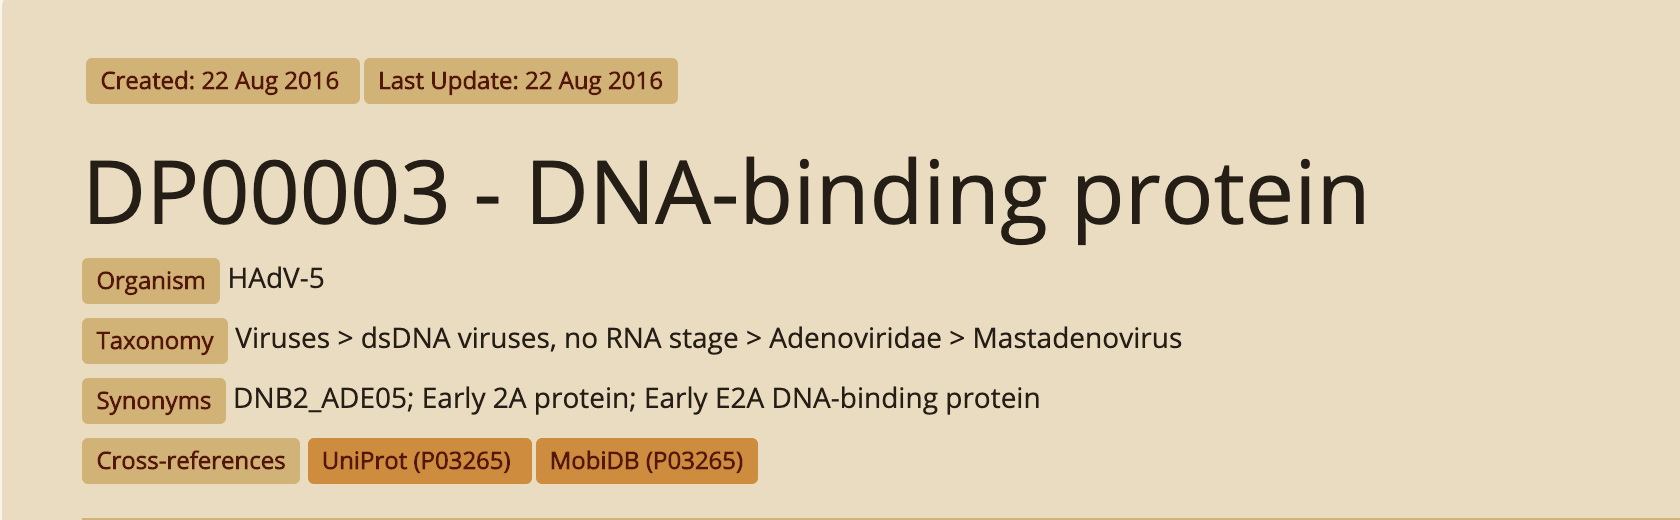
\includegraphics[width=0.7\textwidth]{Figures/App/DisProt.png}
    \caption{Prikaz $DisProt$ baze.}
    \label{fig:DisProt}
\end{figure}

\begin{figure}[H]
	\centering
    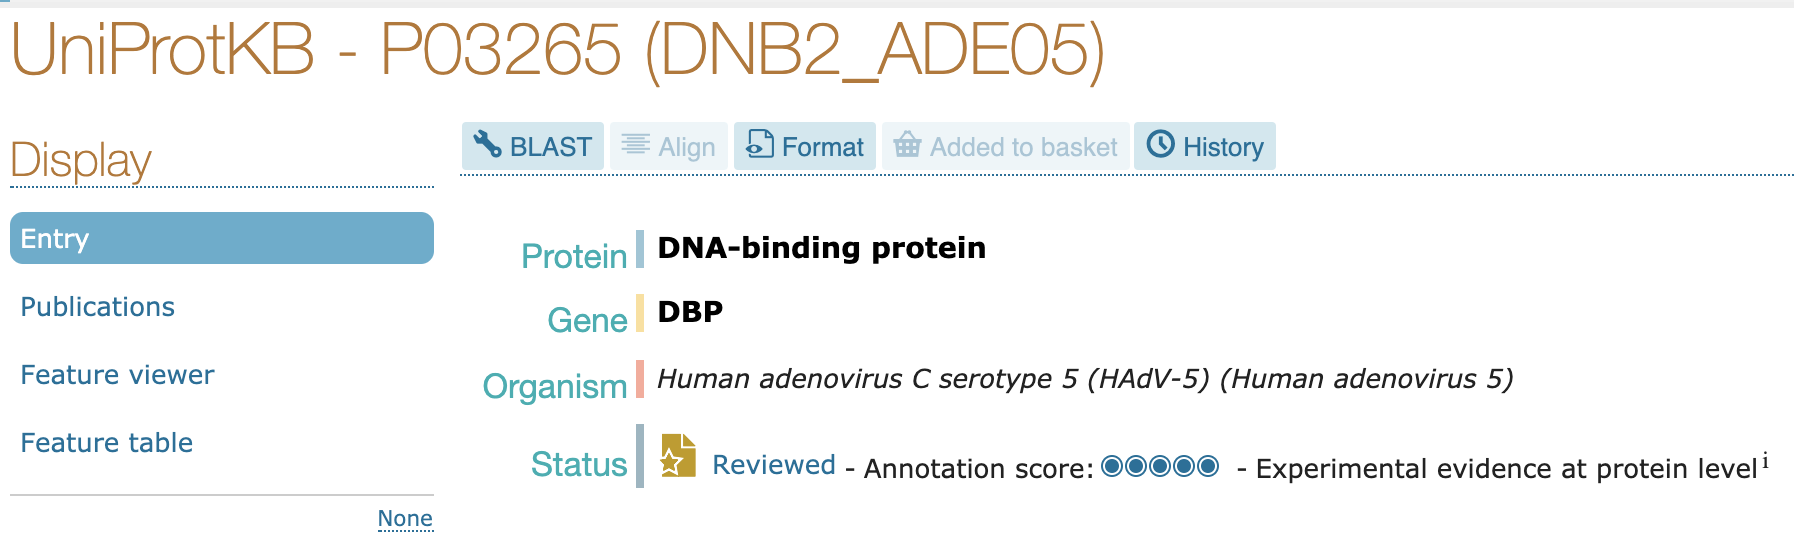
\includegraphics[width=0.7\textwidth]{Figures/App/UniProt.png}
    \caption{Prikaz $UniProt$ baze.}
    \label{fig:UniProt}
\end{figure}

Najpre unose se $identifikator$ i $.fasta$ datoteka u odgovarajuća polja za unos, kao što se može videti na slici \ref{fig:poljaunos}.
\begin{figure}[H]
	\centering
    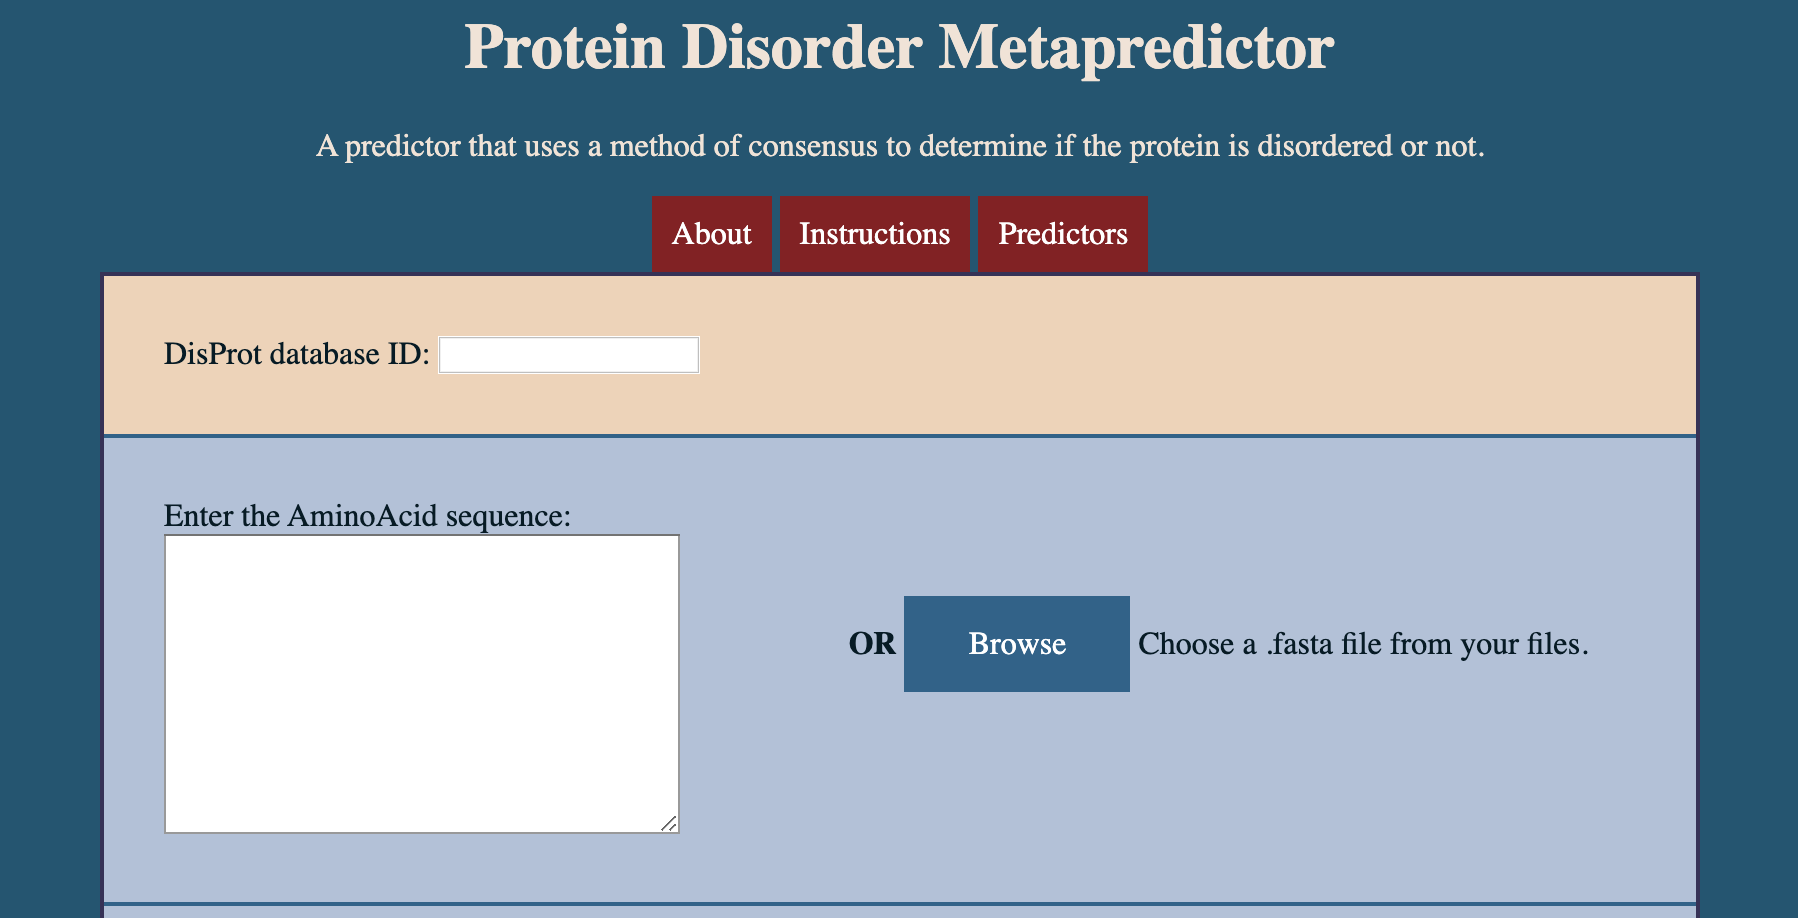
\includegraphics[width=0.7\textwidth]{Figures/App/first_screen.png}
    \caption{Prikaz polja za unos.}
    \label{fig:poljaunos}
\end{figure}
Bira se datoteka sa računara (ili unosi nisku), nakog čega se, ukoliko je niska uneta preko datoteke njen sadržaj prikazuje u tekstualnom polju čime se dobija izgled kao na slici \ref{fig:unos}.
\begin{figure}[H]
	\centering
    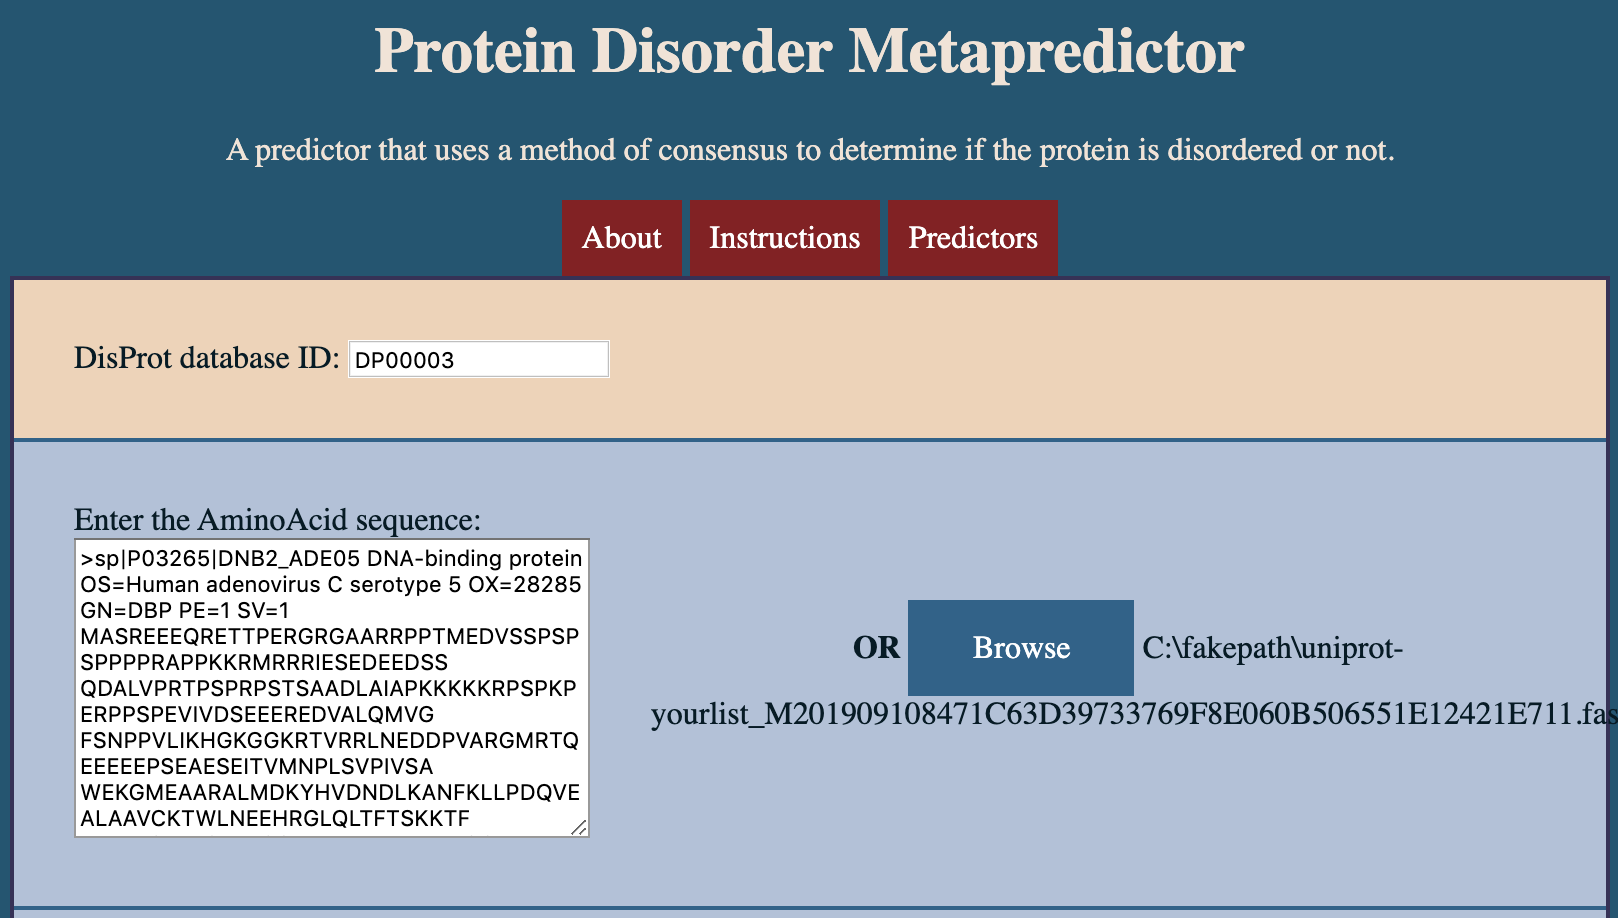
\includegraphics[width=0.7\textwidth]{Figures/App/second_screen.png}
    \caption{Prikaz polja za unos nakon popunjavanja.}
    \label{fig:unos}
\end{figure}
Nakon toga, kretanjem ka dnu strane (prikazano na slici \ref{fig:browse}) nailazi se na spisak dostupnih prediktora, kao i veze ka njihovim zvaničnim stranicama. Klikom na dugme $"$Submit$"$ podaci se šalju na server.
\begin{figure}[H]
	\centering
    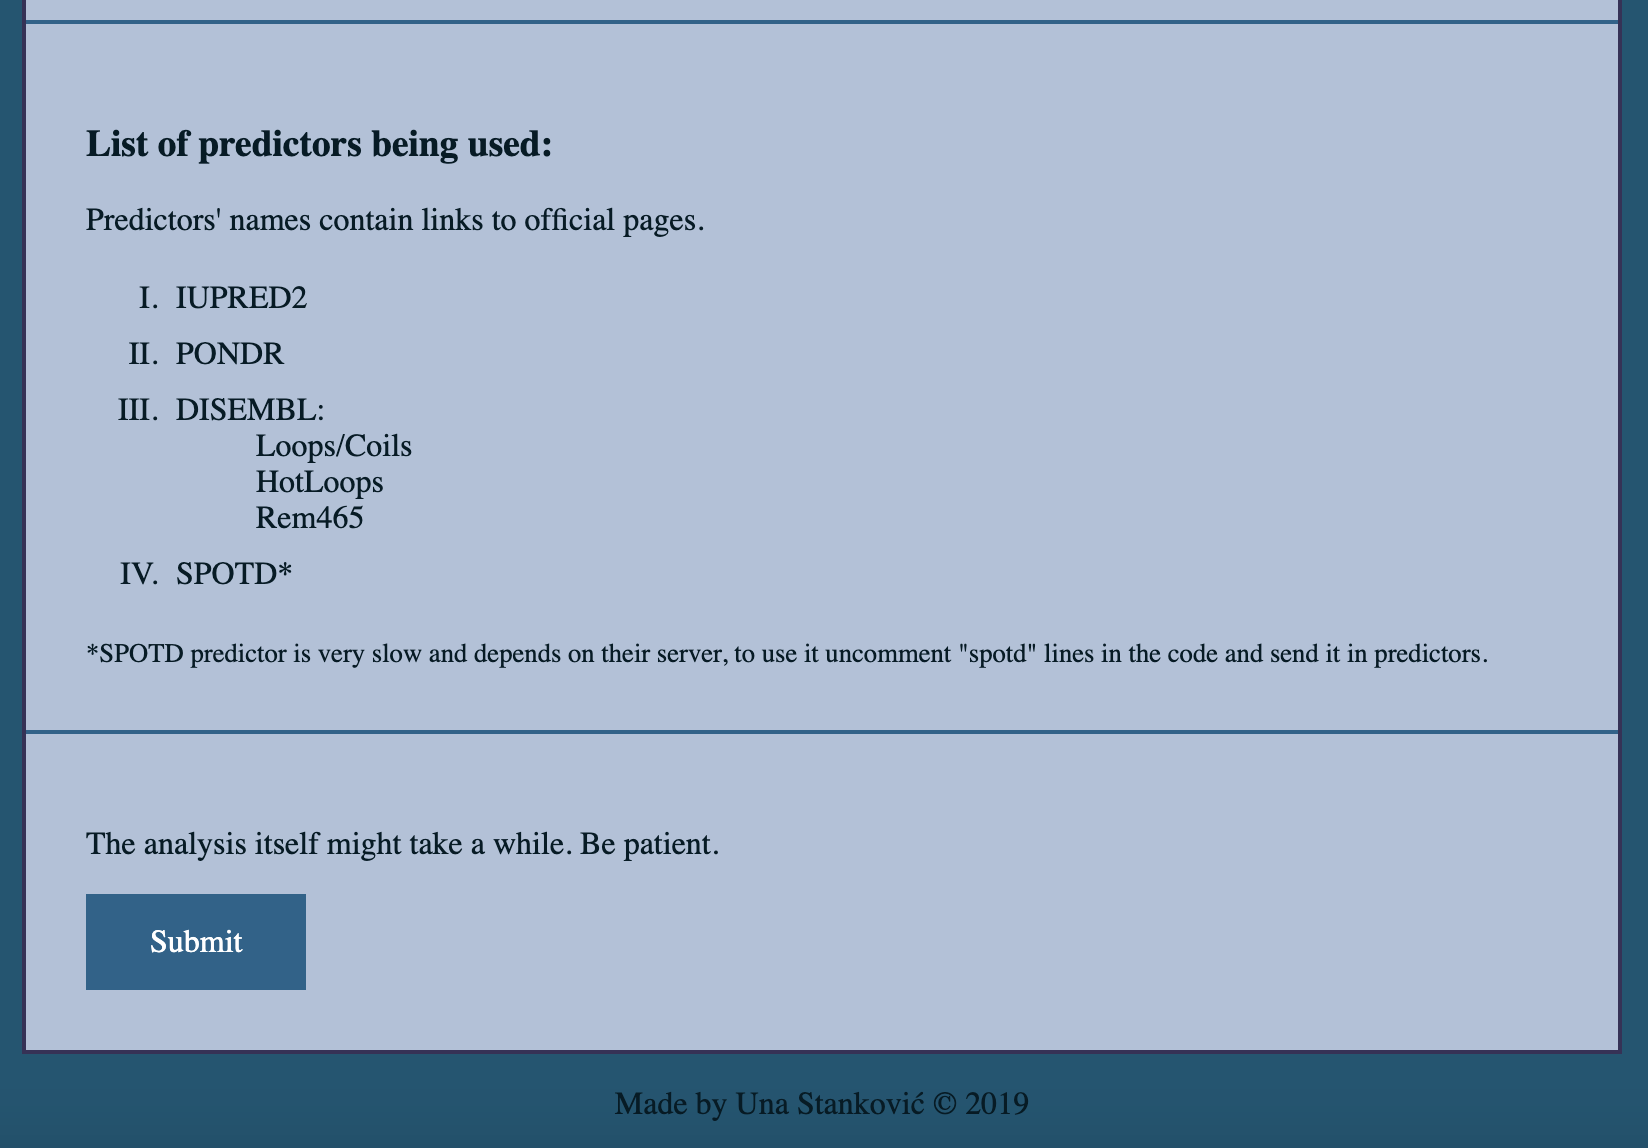
\includegraphics[width=0.7\textwidth]{Figures/App/third_screen.png}
    \caption{Prikaz liste dostupnih prediktora i slanja informacija ka serveru.}
    \label{fig:browse}
\end{figure}
Potrebno je neko vreme da se sva izračunavanja izvrše, a potom se pojavljuje strana sa rezultatima. Sa leve strane navedeni su prediktori koji su učestvovali u davanju odluka, neuređeni regioni iz $DisProt$ baze, kao i konsenzus u vidu brojeva. Procentualno, shodno visini konsenzusa, polje je obojeno u crveno.Prikaz stranice sa opisanim rezultatima nalazi se na slici \ref{fig:results}.
\begin{figure}[H]
	\centering
    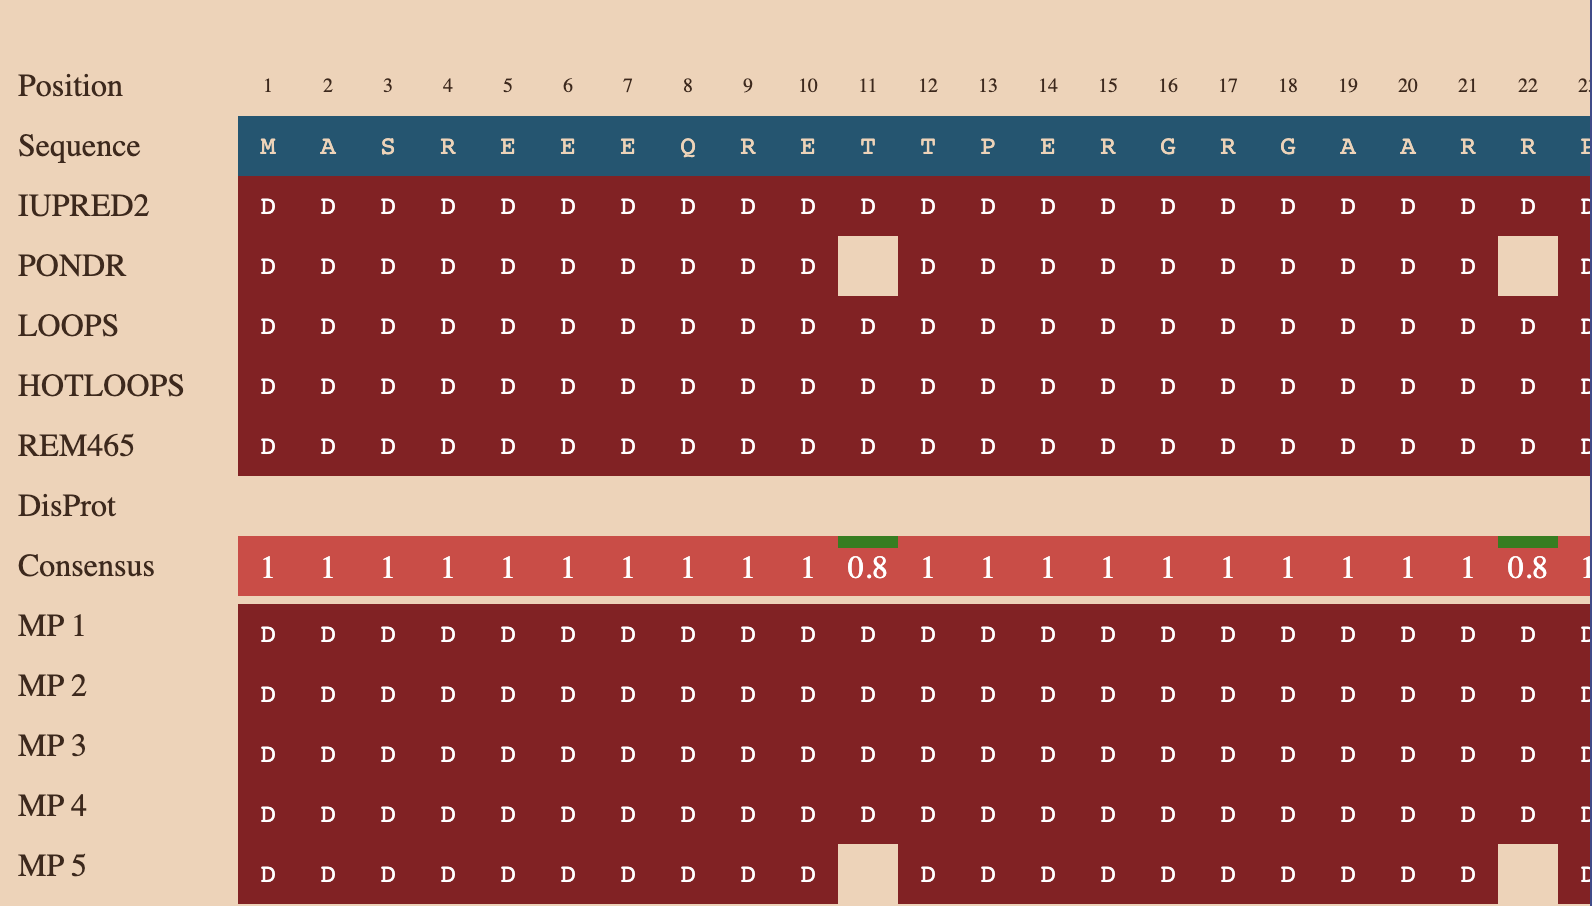
\includegraphics[width=0.7\textwidth]{Figures/App/fourth_screen.png}
    \caption{Prikaz dobijenih rezultata.}
    \label{fig:results}
\end{figure}
Uzimajući u obzir da je dužina sekvenci koja se posmatra obimna i da je nemoguće izvršiti prikaz na samo jednoj dužini stranice, omogućen je pregled cele sekvence, pomeranjem na levo sa dužinom kao što se može videti na slici  \ref{fig:disprotrez}.
\begin{figure}[H]
	\centering
    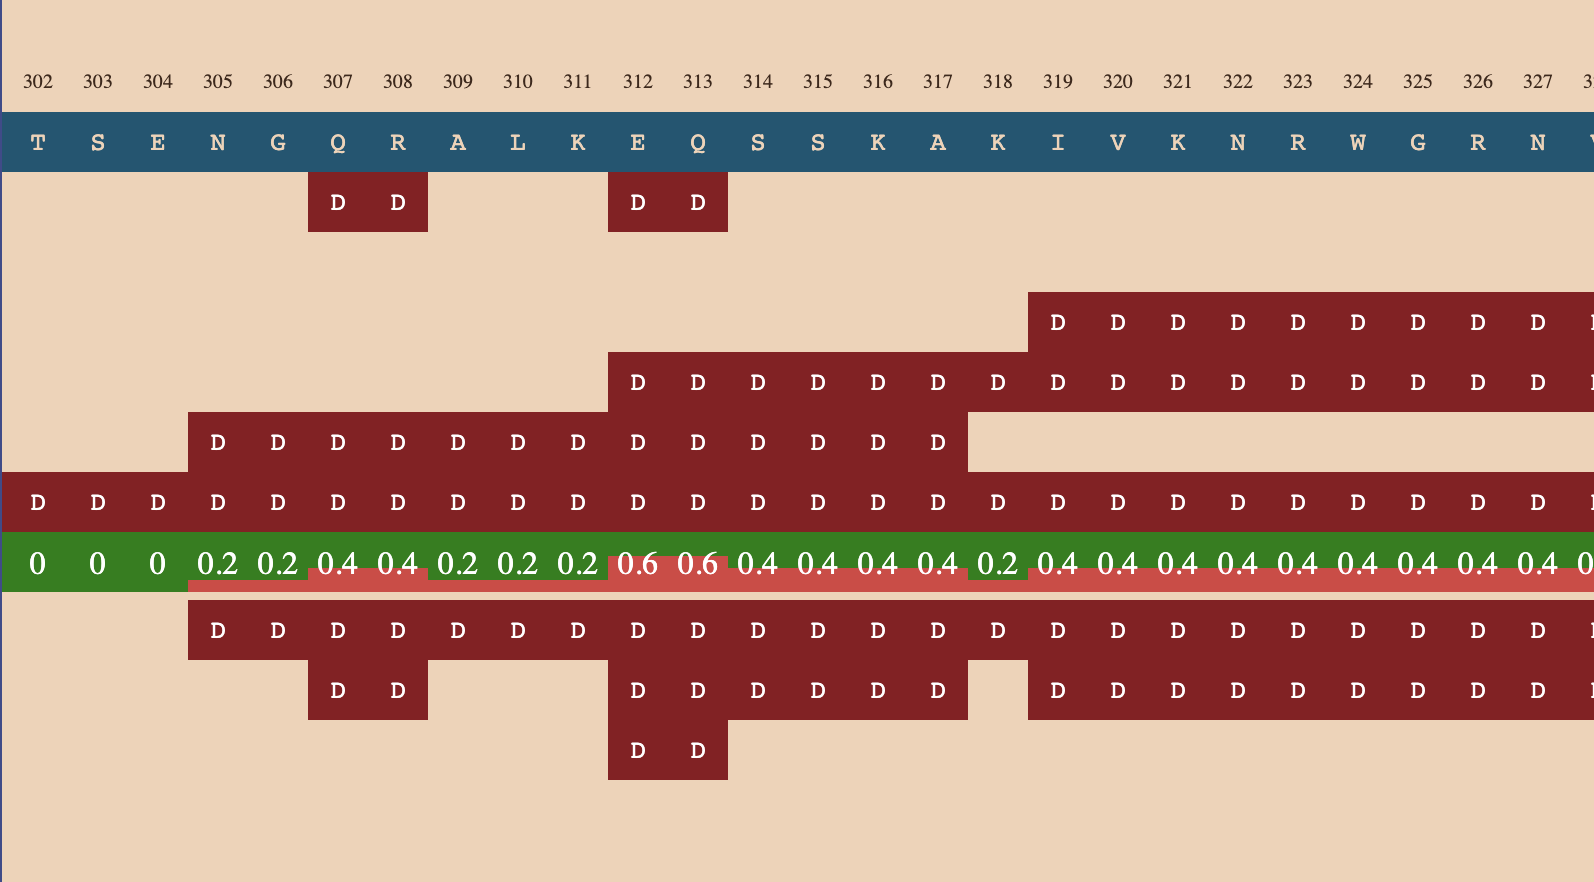
\includegraphics[width=0.7\textwidth]{Figures/App/fifth_screen.png}
    \caption{Prikaz dobijenih rezultata na kom se vidi i izlaz iz $DisProt$ baze.}
    \label{fig:disprotrez}
\end{figure}

Ispod navedenih rezultata nalazi se prikaz vrednosti metrika za dati konsenzus i rezultate iz $DisProt$ baze. U obzir su uzete četiri statističke mere: tačnost, preciznost, odziv i F1 mera. Izgled prikaza ovih metrika vidi se na slici \ref{fig:grafik}

\begin{figure}[H]
	\centering
    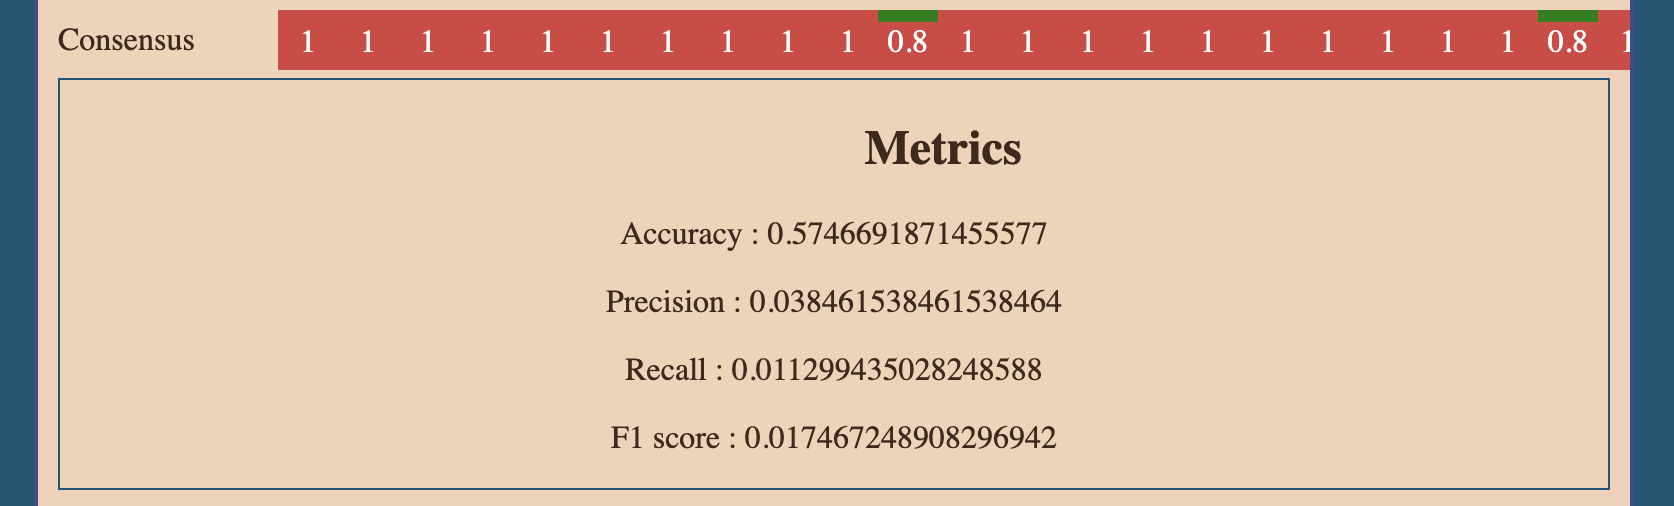
\includegraphics[width=0.7\textwidth]{Figures/App/seventh_screen.png}
    \caption{Prikaz vrednosti metrika.}
    \label{fig:metrike}
\end{figure}

Nakon metrika, sledeća stvar od interesa je grafik neuređenosti na osnovu konsenzusa. Na grafiku se nalazi visina konsenzusa u odnosu na poziciju u sekvenci.
Analizom dobijenih rezultata možemo uvideti oko kojih regiona se prediktori slažu za formirani prag od $0.5$ koji je obeležen crvenom linijom. Prikaz grafika može se videti na slici \ref{fig:grafik}.
\begin{figure}[H]
	\centering
    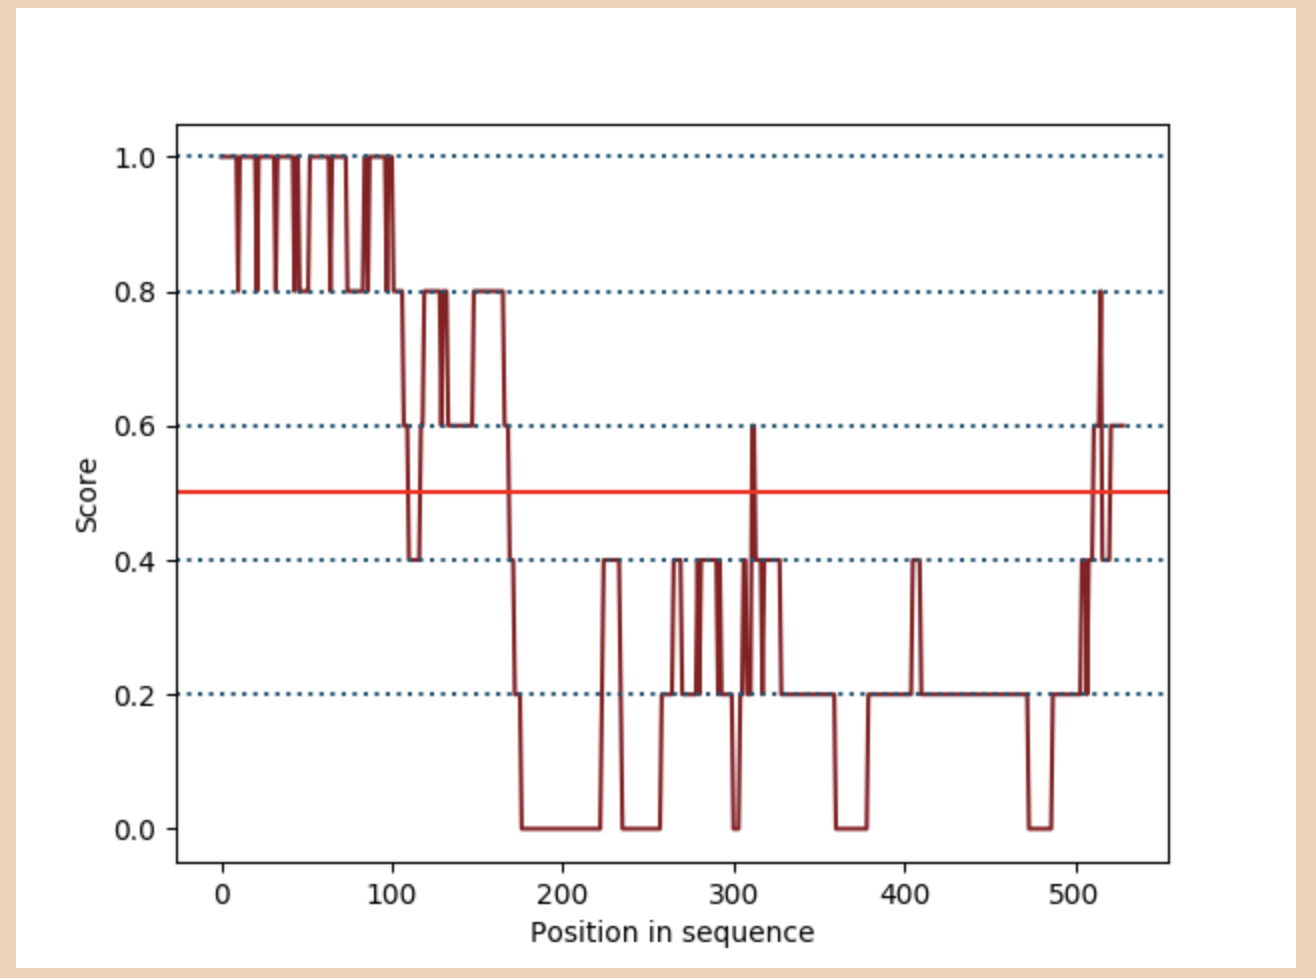
\includegraphics[width=0.7\textwidth]{Figures/App/sixth_screen.png}
    \caption{Prikaz dobijenih rezultata na grafiku.}
    \label{fig:grafik}
\end{figure}

S obzirom da su analizirane i detaljnije metrike, njihov prikaz se vrši na samom dnu strane u vidu tabele prikazane na \ref{fig:detailed}. U tabeli su navedene mere i broj prediktora koji je korišćen.
\begin{figure}[H]
	\centering
    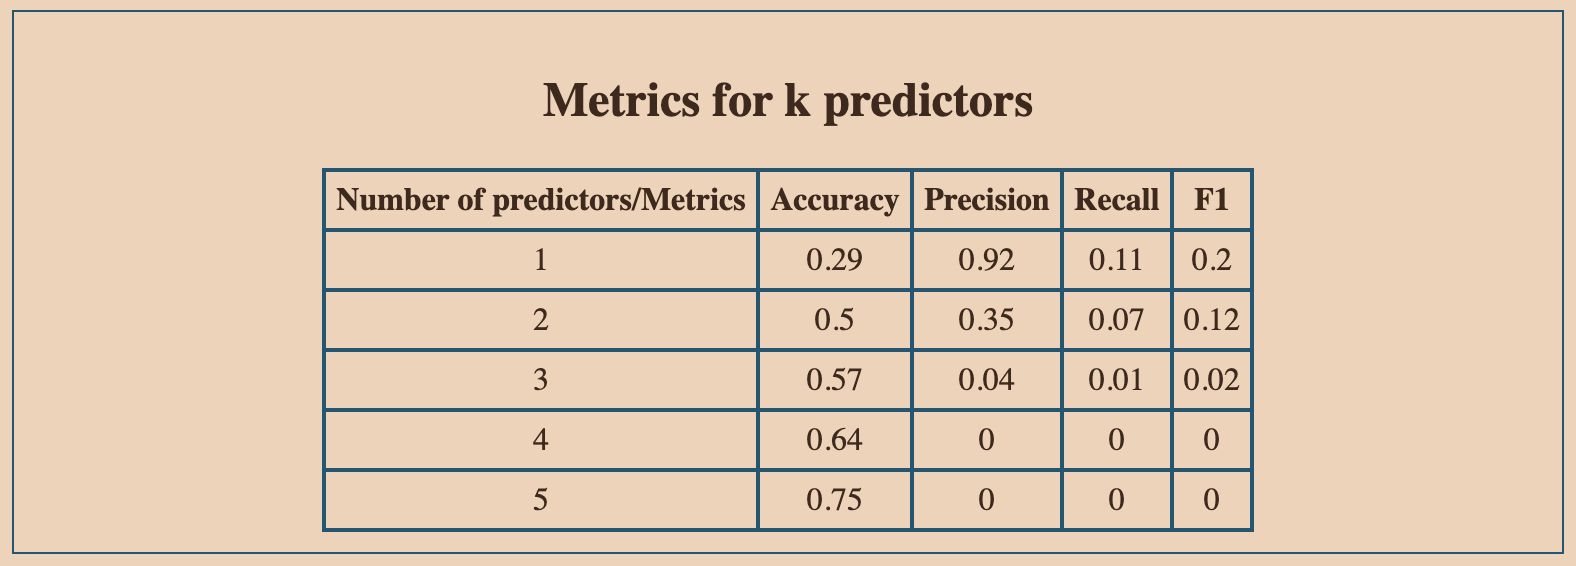
\includegraphics[width=0.7\textwidth]{Figures/App/detailed.png}
    \caption{Prikaz dobijenih rezultata u tabeli.}
    \label{fig:detailed}
\end{figure}


Osim svega navedenog, u vrhu strane nalaze se dugmići koji se odnose na dodatne informacije, kao što su o projektu i uputstvo. Klikom na dugme $About$ dobijaju se detaljnije informacije o autoru, motivacija, cilj i korišćene mere, kao što se može videti na slici \ref{fig:about}. Dok se detaljno uputstvo za korišćenje aplikacije nalazi na stranici koja je prikazana na slici  \ref{fig:instr}.
\begin{figure}[H]
	\centering
    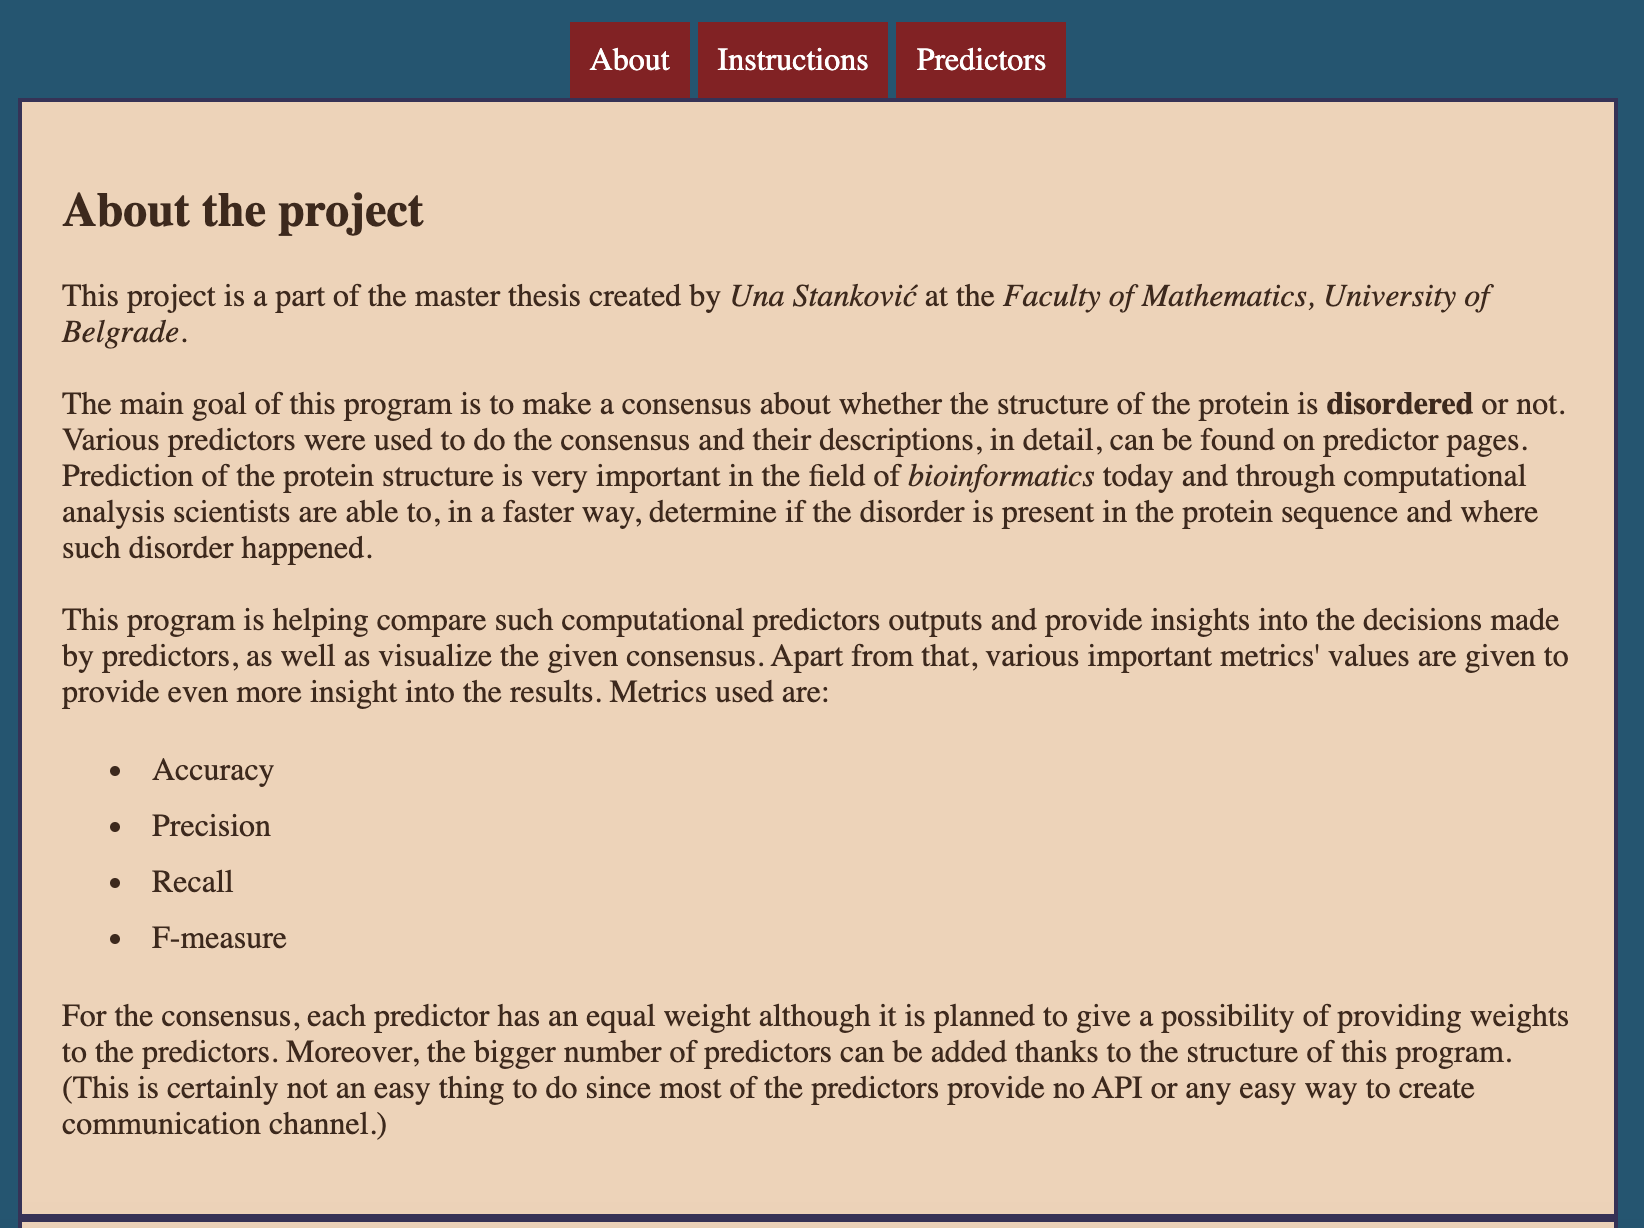
\includegraphics[width=0.7\textwidth]{Figures/App/about.png}
    \caption{Prikaz stranice koja se odnosi na dodatne informacije.}
    \label{fig:about}
\end{figure}
\begin{figure}[H]
	\centering
    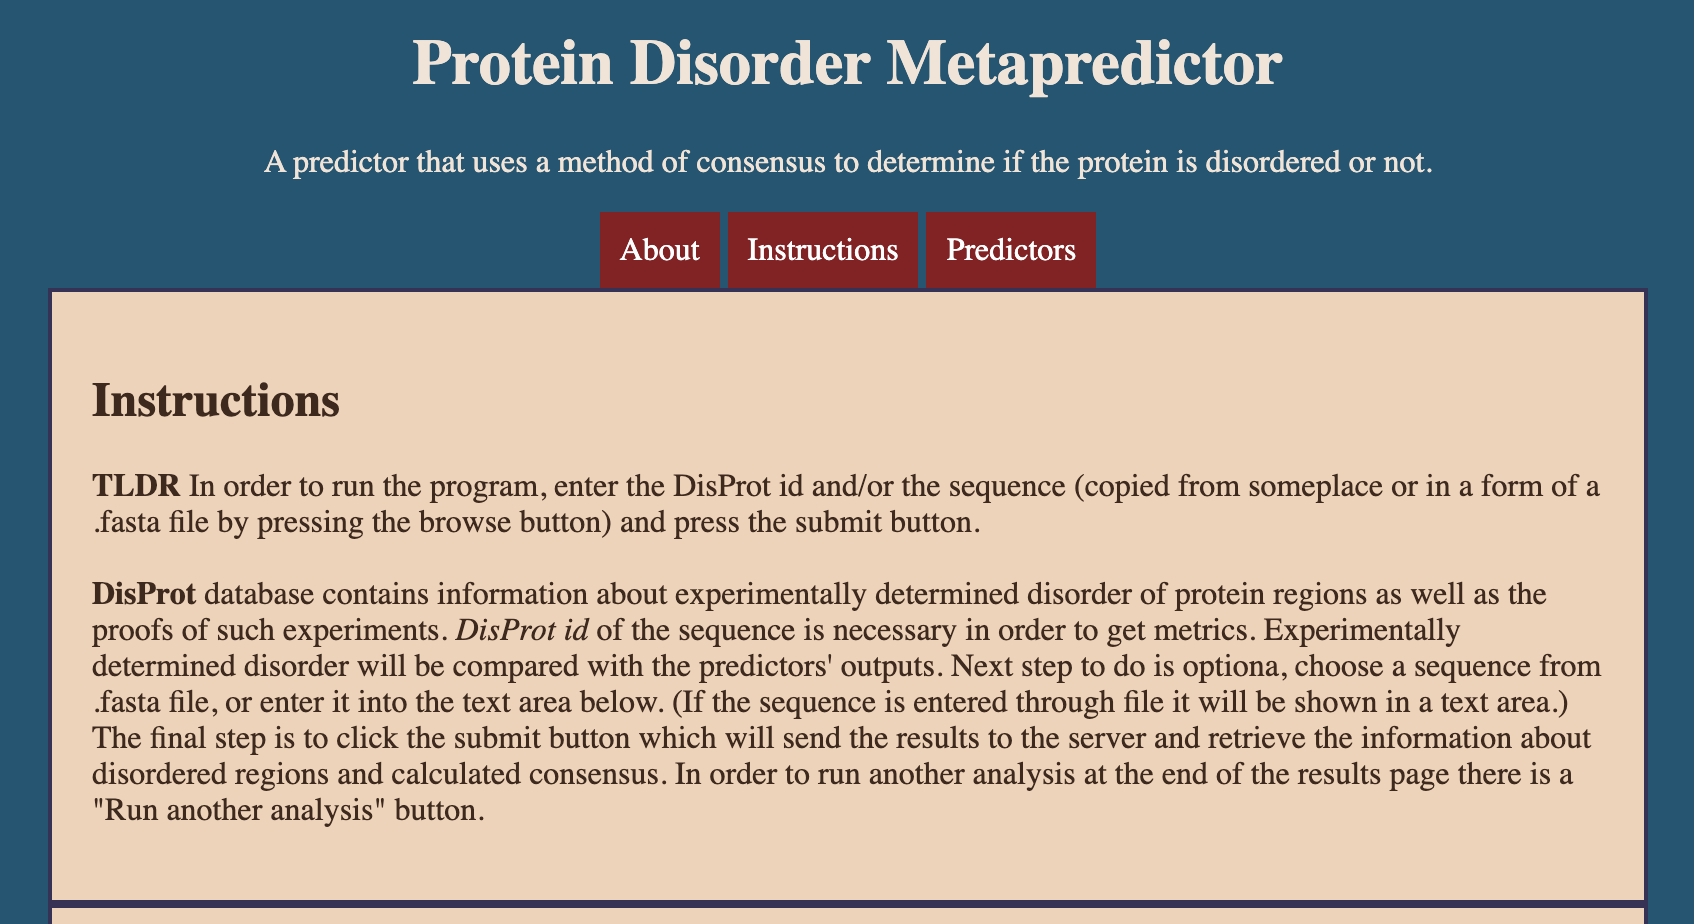
\includegraphics[width=0.7\textwidth]{Figures/App/instructions.png}
    \caption{Prikaz stranice sa uputstvom za korišćenje aplikacije.}
    \label{fig:instr}
\end{figure}

\section{Procena kvaliteta}
Kao što je ranije navedeno, funkcionalnosti ove aplikacije ogledaju se u uporednoj analizi izlaza više prediktora. Osim što se izlazi prediktora mogu uporediti vizuelnim putem, posmatranjem tabele ili grafika, dati su i rezultati nekoliko statističkih mera koje pružaju formalniji uvid u rezultate metaprediktora. 

\subsection{Merenje pouzdanosti metaprediktora}
Kako bi se stekla jasnija slika stanja proteina koje su vratili prediktori neophodno je da osim vizuelnog prikaza postoji i formalno merilo kvaliteta metaprediktora. Da bi se to postiglo korišćene su naredne mere kvaliteta:
\begin{itemize}
\item Preciznost (eng. \em{precision}), 
\item Odziv (eng.  \em{recall}), 
\item Tačnost (eng. \em{accuracy}) i 
\item F-mera (eng. \em{F-measure}). 
\end{itemize} 
Ove mere su veoma pogodne kako bi se utvrdilo koliko dobro metaprediktor predviđa u odnosu na eksperimentalno utvrđenu neuređenost. Poređenje se radi u odnosu na povratne informacije iz $DisProt$ baze.\\\\
U aplikaciji je prikazano dva pristupa korišćenja metrika:
\begin{enumerate}
\item Prvi vid predstavlja prikaz metrika za vrednosti dobijene odnosom onoga što su svi prediktori rekli da je neuređenost (odnosno, konsenzusa koji su dali sa pragom $0.5$) i onoga što je dobijeno iz $DisProt$ baze. Ovim vidom merimo rezultate koje je dao sam metaprediktor. S obzirom na to da se uočava da rezultati nisu uvek sjajni i da se veoma često pojavljuje situacija da, čak i kada se svi prediktori slože da je neki region neuređen, to nije potvrđeno eksperimentalnim putem dolazi se do sledećeg. Prvo, moguće je da regioni za koje su prediktori utvrdili da su neuređeni nisu eksperimentom ni posmatrani. Drugo, moguće je da prediktori sami po sebi nisu dovoljno pouzdani. 
\item Drugi vid predstavlja prikaz metrika za vrednosti dobijene odnosom konsenzusa za $k$ prediktora (može ih biti od $1$ do $5$) i onoga što je dobijeno eksperimentalnim putem. Ovim vidom merimo rezultate dobijene posmatranjem manjeg ili većeg broja prediktora i konsenzusa njihovih odluka. Vrednosti metrika koje se dobijaju ovim putem vrlo često se, posebno za $odziv$ i $F$-meru, svode na $0$ što je i razumljivo s obzirom na to da treba da se uklopi nekoliko faktora. Najpre više od $k$ prediktora treba da kaže za neki region da je neuređen. Potom da bi taj region bio uzet u obzir treba da se poklopi i da je $DisProt$ za taj region rekao da neuređen.  
\end{enumerate}

U tabeli \ref{table:2} nalazi se prikaz metrika za sekvencu sa identifikatorom $DP00003$, dok se u tabeli \ref{table:3} nalazi se prikaz metrika za sekvencu sa identifikatorom $DP00005$. Ove sekvence su odabrane jer predstavljaju jednu prosečnu sekvencu i, bitnije, jednu sekvencu koja je eksperimentalno u potpunosti neuređenea. Iz prikaza ovih vrednosti vidi se da se izlaz rezultata metaprediktora poklapa  poprilično sa onime što je $DisProt$ vratio za sekvencu $DP00005$ u odnosu na sekvencu $DP00003$. Međutim, ako bi se malo bolje obratila pažnja na ono što je vraćeno iz baze i na neuređenost regiona, primećuje se da je sekvenca $DP00005$ cela neuređenaa, čime se dolazi do poprilično zanimljivih rezultata kada se posmatraju metaprediktori. Dolazi se do toga da se vidi rezultat onoga što su metaprediktori dali, praktično nezavisno od $DisProt$ baze. 

\begin{table}[H]
\centering
 \begin{tabular}{||c c c c c||} 
 \hline
 Broj prediktora/Metrika & Tačnost & Preciznost & Odziv & Fmera\\ [0.5ex] 
 \hline\hline
 1 & 0.2854 & 0.9231 & 0.1137 & 0.2025 \\ 
 \hline
 2 & 0.5047 & 0.3462 & 0.0732 & 0.1208 \\
 \hline
 3 & 0.6389 & 0 & 0 & 0 \\
 \hline
 4 & 0.6389 & 0 & 0 & 0\\
 \hline
 5 & 0.7543 & 0 & 0 & 0\\ [1ex] 
 \hline
\end{tabular}
\caption{Prikaz detaljnih metrika za sekvencu DP00003.}
\label{table:2}
\end{table}

\begin{table}[H]
\centering
 \begin{tabular}{||c c c c c||} 
 \hline
 Broj prediktora/Metrika & Tačnost & Preciznost & Odziv & Fmera\\ [0.5ex] 
 \hline\hline
 1 & 0.8879 & 0.8879 & 1 & 0.9406 \\ 
 \hline
 2 & 0.8318 & 0.8318 & 1 & 0.9082 \\
 \hline
 3 & 0.1215 & 0.1215 & 1 & 0.2167 \\
 \hline
 4 & 0.1215 & 01215 & 1 & 0.2167\\
 \hline
 5 & 0 & 0 & 0 & 0\\ [1ex] 
 \hline
\end{tabular}
\caption{Prikaz detaljnih metrika za sekvencu DP00005.}
\label{table:3}
\end{table}
